\documentclass{article}

%PACKAGES
\usepackage{titlesec}	%Section config
\usepackage{titling}	%Calling \theauthor
\usepackage[margin=30mm]{geometry}	%Change margins
\usepackage{array}
\usepackage{graphicx}	% for foto
\usepackage{pdfpages} 	%attachments
\usepackage{caption} 	%supress captions
\usepackage{xcolor}		%for coloring text

\usepackage{hyperref} 	%url
\hypersetup{colorlinks=false}
    
%change fond typeface
\usepackage[T1]{fontenc}
\usepackage{lmodern}

%Section's config
\titleformat{\section}
{\huge}
{}
{0mm}
{\bfseries\lowercase}[\titlerule]
 
\titleformat{\subsection}
{\Large\bfseries}
{\hspace{-4mm}$\bullet$}
{0mm}
{ }

\titlespacing{\subsection}{0mm}{6mm}{0mm}

\titleformat{\subsubsection}[runin]
{\bfseries}
{}
{0mm}
{}[: ]

\titlespacing{\subsubsection}{0mm}{1.5mm}{3mm}

%Title's config
\renewcommand{\maketitle}{
\begin{center}
\raggedleft
{\Huge\bfseries\theauthor}

\vspace{1mm}
{\large\thetitle}

\vspace{10mm}
\end{center}
}

%Struts
\newcolumntype{L}{>{\raggedleft}p{0.13\textwidth}}
\newcolumntype{R}{p{0.8\textwidth}}
\newcommand\VRule{\color{black}\vrule width 0.5pt}

\renewcommand{\labelitemi}{$\textendash$}	%Change bulletpoints

%For attatching
\newcommand{\attach}[3]{
\clearpage
\begin{figure}[b]
	\includegraphics[width=0.90\columnwidth]{#1}
	\centering
    \caption{#2}
    \label{#3}
 
\end{figure}
}

%Change caption
\renewcommand{\figurename}{Ref.}

%Change List of figure's name
\renewcommand{\listfigurename}{attachments}



%=========================MAIN=========================
\begin{document}

\title{\textit{Curriculum Vitae}}
\author{João Pereira}

%Make title with foto
\begin{minipage}{0.65\textwidth}
\begingroup
\maketitle
\endgroup
\end{minipage}
\begin{minipage}{0.3\textwidth}
\flushright{\rotatebox[origin=c]{270}{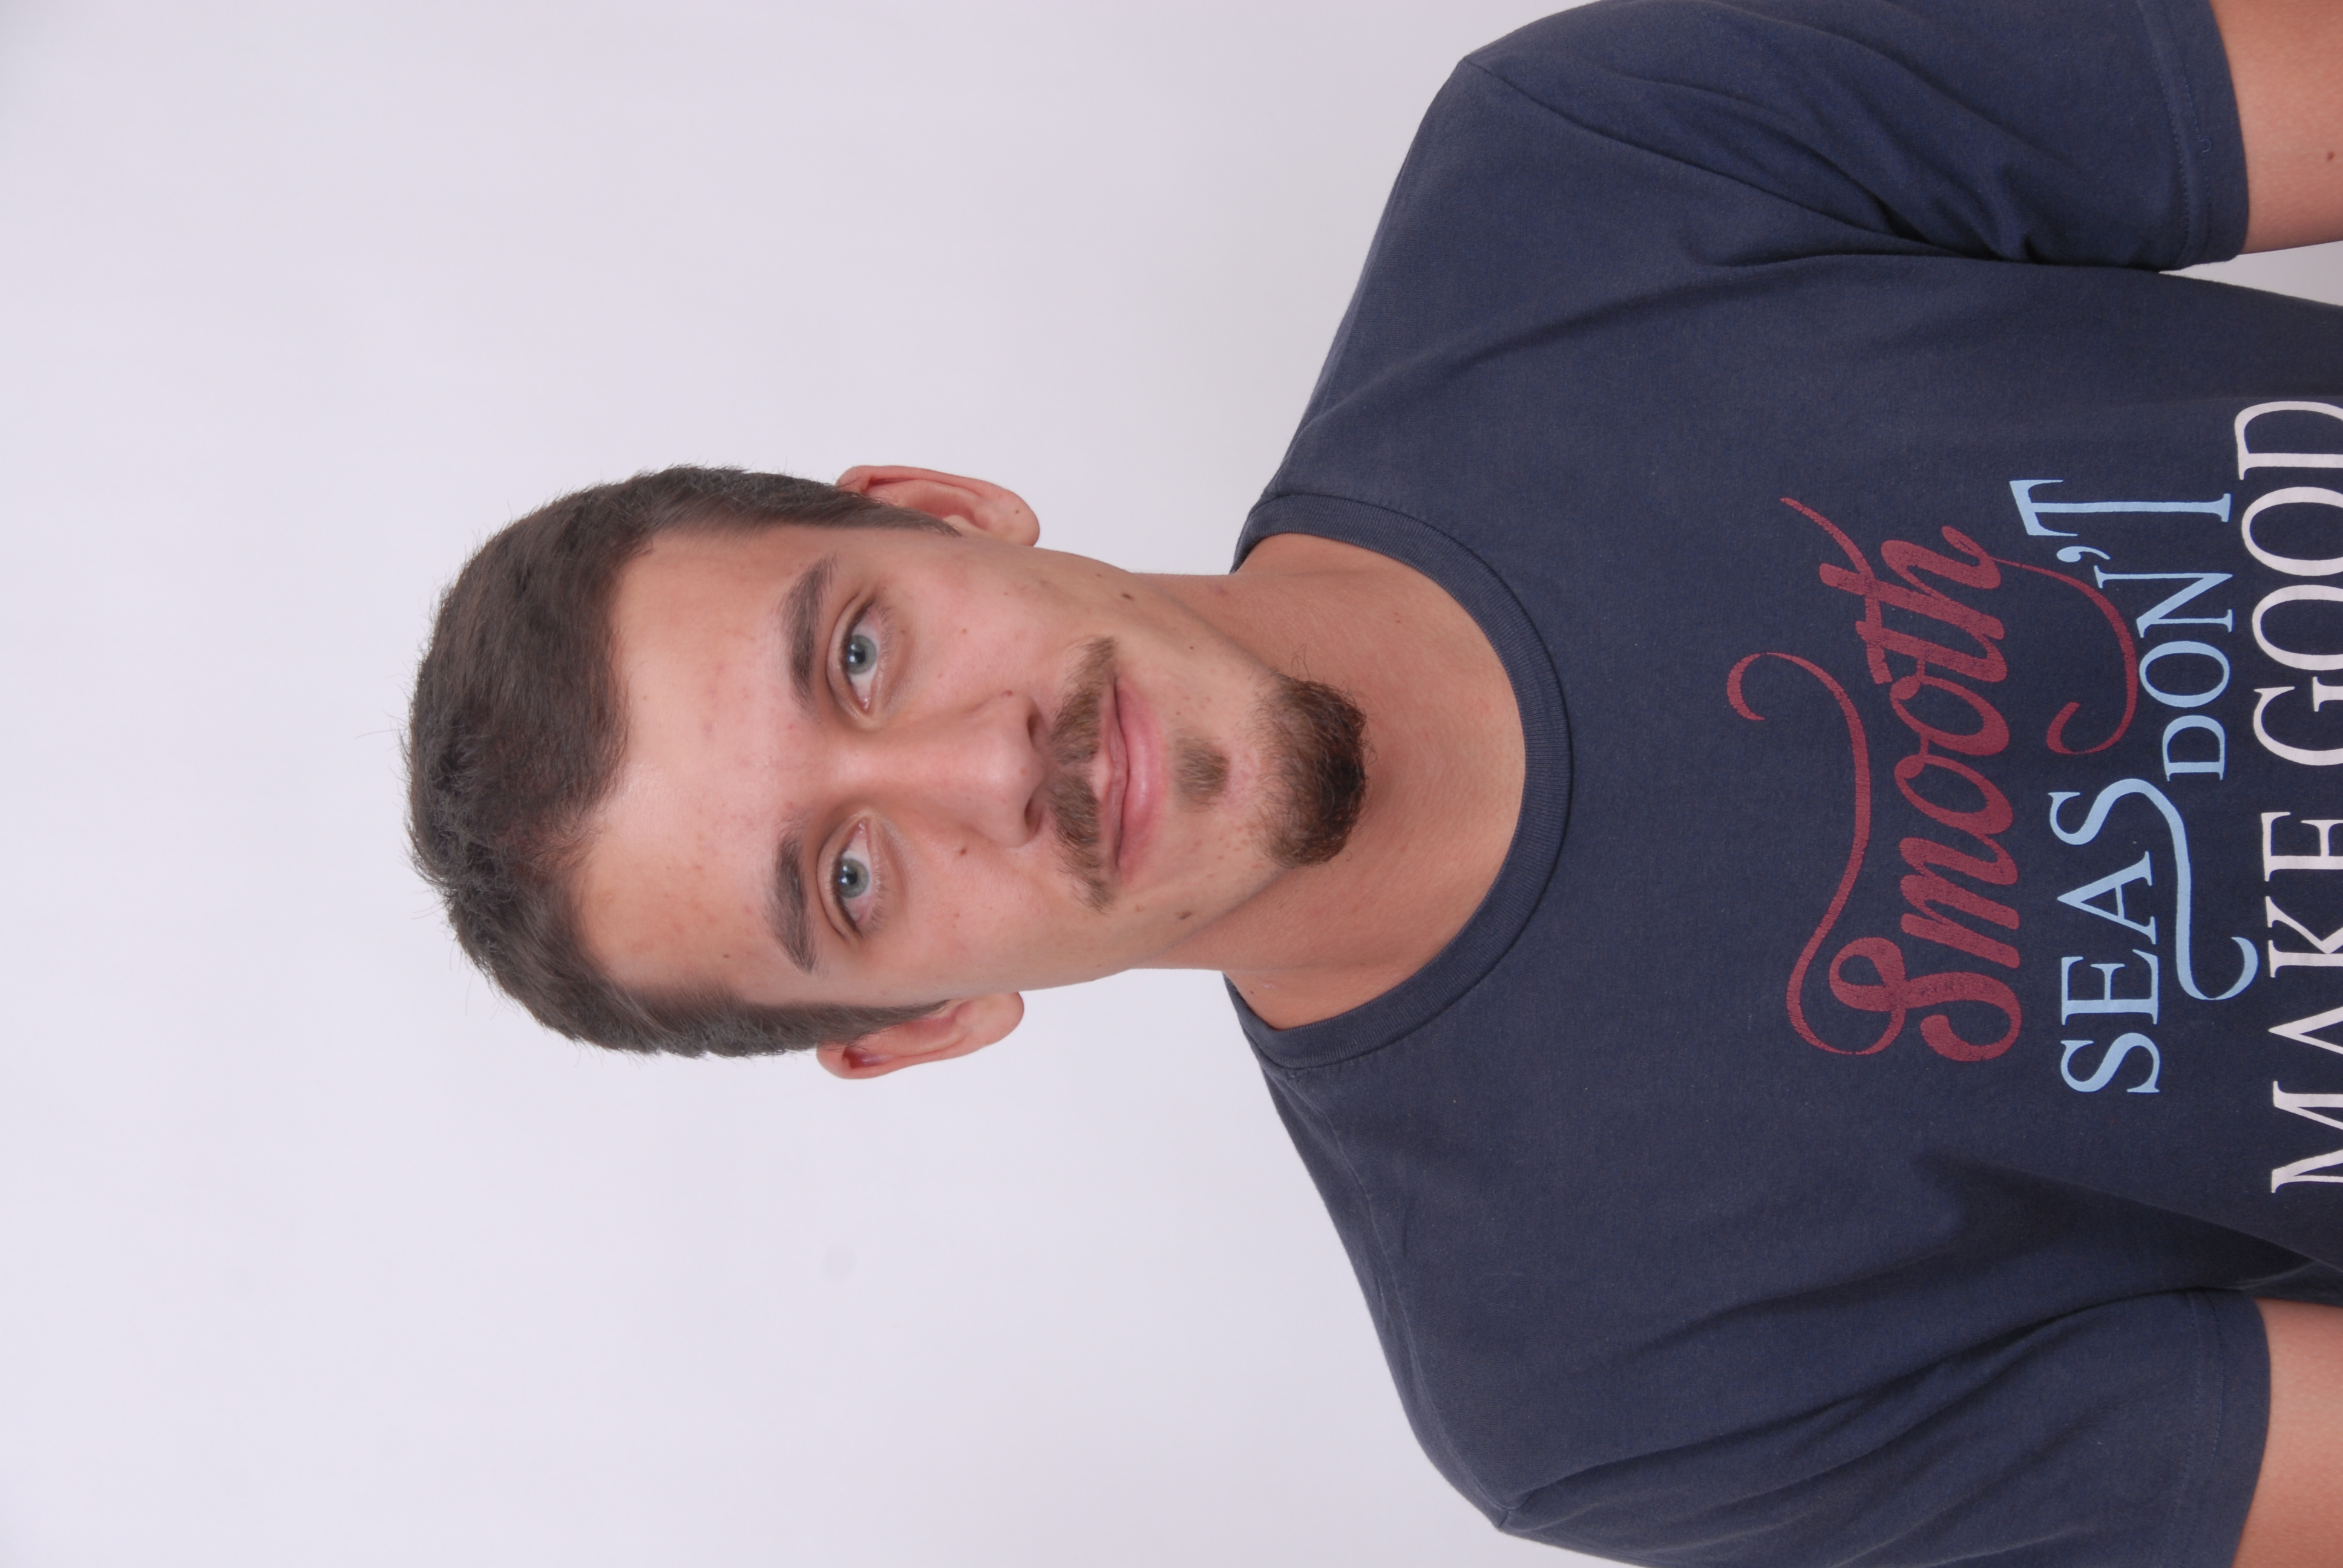
\includegraphics[height=36mm]{Foto_JoaoPereira.jpg}}}
\end{minipage}

%Gray text
\begin{flushright}
{\color{gray}
Source code avaliable at:\\
\url{https://github.com/Pereirajpf/CV_JoaoPereira}\\
(Last updated October 2nd, 2020)
}
\end{flushright}

\section{Personal data}
\subsubsection{Name} 
Freitas Pereira, João Paulo
\subsubsection{Date of birth}
18 September 1996
\subsubsection{Nationality}
Portuguese
\subsubsection{Address}
Estrada Municipal de Ferreiros, Ferreiros, 5000-062 Vila Real, Portugal
\subsubsection{Phone}
+351 966246182
\subsubsection{Email}
pereira.jpf96@gmail.com
\subsubsection{Github}
github.com/Pereirajpf


\section{Academic Education}
\begin{tabular}{L!{\VRule}R}
2019-Present & \textbf{Masters in Bioinformatics and Applications to Life Sciences}, \textit{Universidade de Trás-os-Montes e Alto Douro (Portugal)}\\[8mm]
2015-2019 & \textbf{Batcheler's degree in Biochemistry}, \textit{Universidade de Trás-os-Montes e Alto Douro (Portugal)}\\
& Final grade: 13 (Ref.\ref{Cert})\\
\end{tabular}



\section{Technical Skills}
\subsection{Languages}
\subsubsection{Portuguese}
native speaker
\subsubsection{English}
B2

\subsection{Programing Languages}
\subsubsection{C}
basic
\subsubsection{Python}
intermediate
\subsubsection{Java}
basic
\subsubsection{R}
intermediate
\subsubsection{Matlab}
intermediate

\subsection{Markup Languages}
\subsubsection{\LaTeX}
intermediate
\subsubsection{R Markdown}
intermediate

\section{Conferences attended}
\begin{itemize}
\item I Biochemistry Sessions (UTAD), Vila Real, 15 May 2019 (Ref.\ref{BioSess2019})
\item XII ENEBIOQ / Bioquímica à Beira Ria, Aveiro, 12-15 April 2019 (Ref.\ref{ENEBIOQ2019})
\item Ciência e Cidadania (UTAD), Vila Real 25 February - 1 March 2019 (Ref.\ref{CienciaCidad2019})
\item XI ENEBIOQ, Porto, 23-26 March 2018 ((Ref.\ref{ENEBIOQ2018})
\item Ciência e Cidadania (UTAD), Vila Real, 21-24 November 2017 (Ref.\ref{CienciaCidad2017})
\end{itemize}

\subsection{Workshops}
\begin{itemize}
\item \textit{"Sistemas aquosos bifásicos constituídos por Líquidos Iónicos: da formação à aplicação"}, directed by Dr. Mara G. Freire, integrated in the \textit{XII ENEBIOQ / Bioquímica à Beira Ria}, Aveiro, 12-15 April 2019 (Ref.\ref{ENEBIOQW2019})
\item \textit{"Ferramentas bioquímicas em estudos ambientais: avaliação de efeitos neurotóxicos de poluentes em moluscos"},by Ana Luísa Rebelo, Alexandre Pacheco and Prof. Dra. Lúcia Guilhermino, integrated in the \textit{XI ENEBIOQ}, Porto, 23-26 March 2018 (Ref.\ref{ENEBIOQW12018})
\item \textit{"Como fazer apresentações eficazes"},by Norberto Amaral (TEDxOPORTO, integrated in the \textit{XI ENEBIOQ}, Porto, 23-26 March 2018 (Ref.\ref{ENEBIOQW22018})
\end{itemize}



%\section{Attachments}
\listoffigures

%===============Attachments===============
\attach{attachments/certidão_licenciatura.jpg}{Bachelor's degree completion certificate}{Cert}
\attach{attachments/Ciência_e_cidadania_2017 003.jpg}{Certificate of participation in the event \textit{Ciência e Cidadania}, 2017}{CienciaCidad2017}
\attach{attachments/Ciência_e_cidadania_2019 001.jpg}{Certificate of participation in the event \textit{Ciência e Cidadania}, 2019}{CienciaCidad2019}
\attach{attachments/I_Biochemistry_sessions_2019.jpg}{Certificate of participaton in the event \textit{I Biochemistry sessions}, 2019}{BioSess2019}
\attach{attachments/XIIENEBIOQ_workshops_2019.jpg}{Certificate of participaton in the workshop \textit{"Sistemas aquosos bifásicos constituídos por Líquidos Iónicos: da formação à aplicação"}, 2019}{ENEBIOQW2019}
\attach{attachments/XIIENEBIOQ_2019.jpg}{Certificate of participaton in the event \textit{XII ENEBIOQ / Bioquímica à Beira Ria}, 2019}{ENEBIOQ2019}
\attach{attachments/XIENEBIOQ_2018.jpg}{Certificate of participaton in the event \textit{XI ENEBIOQ}, 2018}{ENEBIOQ2018}
\attach{attachments/XIENEBIOQ_workshop1_2018.jpg}{Certificate of participaton in the workshop \textit{"Ferramentas bioquímicas em estudos ambientais: avaliação de efeitos neurotóxicos de poluentes em moluscos"}, 2018}{ENEBIOQW12018}
\attach{attachments/XIENEBIOQ_workshop2_2018.jpg}{Certificate of participaton in the workshop \textit{"Como fazer apresentações eficazes"}, 2018}{ENEBIOQW22018}

\end{document}